\documentclass[tikz,border=2pt]{standalone}
\usepackage{amsmath,amssymb}
\usepackage{tikz}
\usetikzlibrary{arrows.meta}

\begin{document}
% De Moivre: raising a point of the unit circle to the n-th power multiplies its angle by n.
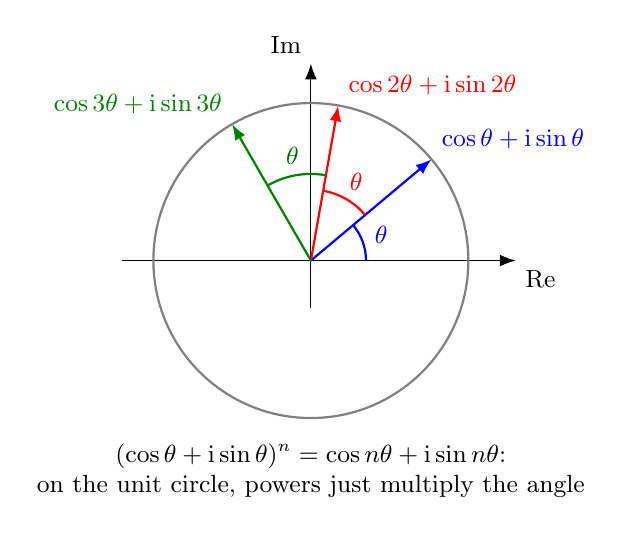
\begin{tikzpicture}[every node/.style={font=\small}, >={Latex[length=2mm]}]
	\draw[->] (-2.4,0) -- (2.6,0) node[below right] {$\mathrm{Re}$};
	\draw[->] (0,-0.6) -- (0,2.5) node[above left] {$\mathrm{Im}$};
	\draw[gray, thick] (0,0) circle (2);
	\draw[->, blue, thick] (0,0) -- (40:2) node[above right] {$\cos\theta+\mathrm{i}\sin\theta$};
	\draw[->, red, thick] (0,0) -- (80:2) node[above right] {$\cos2\theta+\mathrm{i}\sin2\theta$};
	\draw[->, green!50!black, thick] (0,0) -- (120:2) node[above left] {$\cos3\theta+\mathrm{i}\sin3\theta$};
	\draw[blue, thick] (0.7,0) arc (0:40:0.7);
	\node[blue, font=\small] at (20:0.95) {$\theta$};
	\draw[red, thick] (40:0.9) arc (40:80:0.9);
	\node[red, font=\small] at (60:1.15) {$\theta$};
	\draw[green!50!black, thick] (80:1.1) arc (80:120:1.1);
	\node[green!40!black, font=\small] at (100:1.35) {$\theta$};
	\node[anchor=north, align=center] at (0,-2.2) {$(\cos\theta+\mathrm{i}\sin\theta)^n=\cos n\theta+\mathrm{i}\sin n\theta$:\\ on the unit circle, powers just multiply the angle};
\end{tikzpicture}
\end{document}
